\clearpage
\section{Back-end dokumentasjon}
\subsection{Installasjon}
Startet med å laste ned laravel, xampp og Gitkraken til datamaskinen. Gjorde clone til repositoren som ble opprettet tidligere i github. Repositoren inneholder laravel. 

\subsection{Database}
Opprettet en database til prosjektet på phpMyAdmin og satt inn databasen og innloggingsinformasjonen i konfigurasjonsfilen .env. Så laget det modeller for databasen. Modellene lages ved å skrive koden nede i kommandolinjen. 
\begin{lstlisting}[language=PHP]
    Php artisan make:model Modelnavn -m
\end{lstlisting}  
Det siste “-m” brukes for å opprette migrasjon for modellen  samtidig. Dette dropes og opprettes etter på: 
 \begin{lstlisting}[language=PHP]
    Php artisan make:migration tabellnavn.
\end{lstlisting}
Etter modellene og migrasjonene er på plass kan det lages felter på tabellene og ta migrasjon for å legge til tabellene til phpMyAdmin. Legge til migrasjonene til phpMyAdmin ved å sette koden Php artisan migrate  i kommandolinjen.
AppServiceProvider defualtlength satt til varchar(255). Dette gjøres for å bestemme lengden på strengen.
Oppretting av  attributter på tabellene gjøres slik: 

\begin{lstlisting}[language=PHP]
    $table->type('atributtnavn');
\end{lstlisting}

Brukte UUID som primære nøkler på de fleste  tabellene. UUID (Universally unique identifier) er en ID som kan gis til tabellrader for å identifisere dem på en måte som er litt finere enn et sekvensielt tabell-ID. \footnote{\url{https://medium.com/binary-cabin/automatically-generating-a-uuid-on-your-laravel-models-b8b9c3599e2b}} Dette hjelper å har større tabellrader enn å bruke increments.

\subsection{Feil under migrasjon}
Prøvde å ta migrasjon oppsto en feilmelding.
\begin{lstlisting}[language=PHP]
Illuminate\Database\QueryException : SQLSTATE[42000]: Syntax error or access violation: 1071 Specified key was too long; max key length is 767 bytes (SQL: alter table `users` add unique `users_email_unique`(`email`))
\end{lstlisting}
Årsaken var at datamaskinen har gammel versjon av mysql som ikke støtter standard streng lengde på 255. Da måtte streng lengden endre til 191 og løste feilen.

\subsection{Lage forhold mellom modellene}
Opprettet relasjoner mellom database-modellene. 
Relasjoner  lages ved å bruke  manyToMany,(belongsToMany), One to One(hasOne), Many to One(belongsTo) og  One to Many (hasMany). Eks.  slik  

\begin{lstlisting}[language=PHP]
    $this->hasMany('App\Model') og invers.
\end{lstlisting}

\subsection{Lagringstest til DB}
Etter jeg opprettet ferdig koblingene mellom modellene, tok jeg test for å lagre data på databasen.Testen gjorde på alle tabellene.

\subsection{Feilmeldinger}
\subsubsection{Felt har ikke  standardverdi}
Fremmednøkkel feltet har ikke  standardverdi.

\begin{lstlisting}[language=PHP]
    SQLSTATE[HY000]: General error: 1364 Field 'id' doesn't have a default value (SQL: insert into `fields` (`name`, `slug`, `updated_at`, `created_at`) values (HELLO WORLD, hello_world, 2019-02-06 08:57:48, 2019-02-06 08:57:48))
\end{lstlisting}

Feilen oppsto da fremmednøkkel feltet ble satt til null. Dette løste ved å sette riktig verdien til feltet eller sette fremmednøkkelen til nullable. 

\subsubsection{Data truncated for column}
Vi bruker UUID i stedet increments og trenger å identifisere primærnøkkelen slik.
\begin{lstlisting}[language=PHP]
    $table->uuid('id')->primary();
\end{lstlisting}

For å bruke UUID er det viktig å opprette UsesUuid.php trait i App / Trait.
Denne filen brukes til å opprette UUID automatisk når du oppretter nye modeller, deaktivere automatisk increments id-er, sette primærnøkkel som uuid og sette primærnøkkeltype som streng.\footnote{
\url{https://medium.com/@mamreezaa/use-uuid-in-lumen-d47ec02c330}}
Siden det ikke opprettet UsesUuid.php trait i App/Trait dukket opp feilmelding. 

\begin{lstlisting}[language=PHP]
SQLSTATE[HY000]: General error: 1364 Field 'id' doesn't have a default value (SQL: insert into `fields` (`name`, `slug`, `updated_at`, `created_at`) values (HELLO WORLD, hello_world, 2019-02-06 08:57:48, 2019-02-06 08:57:48))
\end{lstlisting}
Dette betyr at det prøvde å sende UUID verdi i integer.
Dette ble løst med å lage en trait som automatisk lager en UUID når man lagrer modell til DB. (Filsti: /App/Traits/UsesUUID.php).\footnote{\url{ https://dev.to/wilburpowery/easily-use-uuids-in-laravel-45be.}}
 
\subsubsection{Fremmednøkkel feil}
Feilmeldingen oppsto da det ble prøvd å lagre en bruker på databasen. 

\begin{lstlisting}[language=PHP]
    SQLSTATE[23000]: Integrity constraint violation: 1452 Cannot add or update a child row: a foreign key constraint fails (`sirkus-media`.`users`, CONSTRAINT `users_image_id_foreign` FOREIGN KEY (`image_id`) REFERENCES `images` (`id`)) (SQL: insert into `users` (`name`, `phone`, `email`, `password`, `image_id`, `verified`, `email_token`, `id`, `updated_at`, `created_at`) values (Bere, 4578891, berg@gmail.com, 1234567r, 2432479, 1, e-token, 53f98032-f9bf-40a6-9d70-ca9c0785d7ee, 2019-02-08 10:11:16, 2019-02-08 10:11:16))
\end{lstlisting}

Grunnen var at det ikke går an å sette verdi på en fremmednøkkel felt som verdien ikke finnes på referanse tabellen. Løste ved å sette riktig verdi.

\subsubsection{Fremmednøkkel er ikke satt riktig}
Feilmelding oppsto da migrasjonen utføres. 
Årsaken var at primær og fremmed nøklene satt på ulike type.
Dette betyr at primær nøkkelen blir satt på auto increments og den er unsignedInteger. Da det blir brukt som fremmed nøkkel på en annen tabell burde ha samme type. Dette var satt på integer.
Løste ved å endre typen integer til unsigned integer til fremmednøkkelen. Slik:

\begin{lstlisting}[language=PHP]
    $table->integer('image_size_id')->unsigned();
    $table->foreign('image_size_id')->references('image_size_id')->on('image_sizes');
\end{lstlisting}

\subsubsection{Feilmelding om oppdatering og oppretting kolloner}
\begin{lstlisting}[language=PHP]
    "SQLSTATE[42S22]: Column not found: 1054 Unknown column 'updated_at' in 'field list' (SQL: insert into `image_sizes` (`name`, `max_width`, `max_height`, `id`, `updated_at`, `created_at`) values (size-name, 10, 20, 879d1360-9a74-46f8-b383-ff6ec6e0f387, 2019-02-07 21:08:09, 2019-02-07 21:08:09))
\end{lstlisting}
Grunnen var at timestamps som oppretter opprettings- og oppdateringstiden er automatisk aktivert.
Løste ved å deaktivere den. Slik: 

\begin{lstlisting}[language=PHP]
    public $timestamps = false;
\end{lstlisting}

\subsubsection{Auto Increments feil}
Feilmeldingen sa at fremmednøkkel var ikke satt riktig.
Dette var at auto increments er unsigned integer og brukte bare integer da jeg satte den som fremmednøkkel.
Løste ved å endre integer til UnsignedInteger ved fremmednøkkelen. Slik:

\begin{lstlisting}[language=PHP]
    $table->integer('image_size_id')->unsigned();
    $table->foreign('image_size_id')->references('image_size_id')->on('image_sizes');
\end{lstlisting}

\subsubsection{Forelder/barn fremmednøkkel feil}
Fremmednøkkelen var satt på samme måte som i andre tabeller i et barn tabell. Problemet var at jeg prøvde å lage fremmednøkkel til en tabell som ikke er opprettet enda.
Måtte bryte dette inn i to Schema-blokker, en skaper kolonnene, den andre legger til fremmednøkkel.\footnote{\url{https://stackoverflow.com/questions/18427391/laravel-migration-self-referencing-foreign-key-issue}}
Løste ved å sette fremmednøkkelen på riktig måte. Slik
\begin{lstlisting}[language=PHP]
Schema::create('components', function (Blueprint $table)
       {
           $table->uuid('id')->primary();
           $table->string('name');
           $table->string('slug');
           $table->integer('order');
           $table->uuid('parent_id')->nullable();
           $table->timestamps();
       });
       Schema::table('components', function(Blueprint $table){
           $table->foreign('parent_id')->references('id')->on('components');
       });
\end{lstlisting}

\subsection{Modelkobling test}
Flere fremmednøkkel-felter var satt til nullable som ikke skulle nullable. Startet med å fikse de feltene som skulle ikke ha nullable fremmednøkler.

\subsubsection{Ukjent kolonne feilmelding}
Siden forholdene mellom modellene var ikke satt riktig, oppsto feil under testingen.
\begin{lstlisting}[language=PHP]
"SQLSTATE[42S22]: Column not found: 1054 Unknown column 'links.menu_link_id' in 'where clause' (SQL: select * from links where links.`menu_link_id` = 3 and links.`menu_link_id` is not null) 
\end{lstlisting}
Løste ved å gå gjennom alle modellene og fikse forholdene mellom dem.

\subsection{Roller og Permisjoner}\footnote{\url{https://github.com/spatie/laravel-permission}}
Laravel permisjon er en pakke med tillatelser og roller. Dette hjelper brukere til å knytte seg til tillatelser og roller. Hver rolle er knyttet til flere tillatelser. En rolle og en tillatelse er vanlige Eloquent-modeller\footnote{\url{https://scotch.io/tutorials/user-authorization-in-laravel-54-with-spatie-laravel-permission}}.
\subsubsection{Laravel permisjon pakke installasjon} 
Laravel permisjon pakken er bygget ut over laravel autorisasjon funksjoner\footnote{\url{https://laravel-news.com/two-best-roles-permissions-packages}}.
For installere permisjon pakken kjørte jeg composer require spatie/laravel-permission i kommando linje.

\subsubsection{Inkludere pakken på service provider listen}
Inkluderte permisjon pakken på config/app.php. 
\begin{lstlisting}[language=PHP]
    Spatie\Permission\PermissionServiceProvider::class
\end{lstlisting}

\subsubsection{Publisere migrasjonen}
Ved å kjøre koden på kommandolinjen publisere migrasjon filen for permisjon pakken.
\begin{lstlisting}[language=PHP]
   php artisan vendor:publish --provider="Spatie\Permission\PermissionServiceProvider" --tag="migrations" 
\end{lstlisting}

Siden vi bruker uuid som primær nøkkel på user måtte det redigeres permisjon filen. På permisjon filen er satt 'unsignedBigInteger' som standard og burde det  endres  til uuid. Redigeringen gjøres ved å åpne permisjon filen  under 'database/migrations' og erstatte 'unsignedBigInteger' med 'uuid'.
\begin{lstlisting}[language=PHP]
  $table->unsignedBigInteger($columnNames['model_morph_key'])
    Erstatter med 
 $table->uuid($columnNames['model_morph_key'])
\end{lstlisting}

\subsubsection{Publisere konfigurasjonen}
Konfigureringsfilen tillater oss å angi plasseringen av Eloquent-modellen til permisjon og rolle klasse.
For å publisere konfigurasjonsfilen for pakken kjøres koden nede i kommandolinjen.

\begin{lstlisting}[language=PHP]
  php artisan vendor:publish --provider="Spatie\Permission\PermissionServiceProvider" --tag="config"
\end{lstlisting}

\subsubsection{Bygge opp tabeller}
Tok migrasjon slik permisjon tabellene blir bygget på databasen.
Kjørte koden i kommandolinjen.
\begin{lstlisting}[language=PHP]
  php artisan migrate
\end{lstlisting}

\subsection{Lage API}
For å lage api opprettet det først controller\footnote{\url{https://laravel.com/docs/5.7/controllers}} via cmd terminalen.
Gjøres slik:
\begin{lstlisting}[language=PHP]
    php artisan make:controller PageController --resource
\end{lstlisting}
Den siste parameteren "resource" er et alternativ og kan dropes.

På api.php i routes\footnote{\url{https://laravel.com/docs/5.7/routing}}  registrer det API-ruter.
For alle pages:
\begin{lstlisting}[language=PHP]
    Route::get('/pages', 'PageController@index');
\end{lstlisting} 
For en enkel page:
\begin{lstlisting}[language=PHP]
    Route::get('pages/{page}', 'PageController@show');
\end{lstlisting}

\subsection{API Test}
Brukte en verktøy som heter Postman\footnote{\url{https://www.getpostman.com/product}} for api test. Postman er en HTTP-klient som sender en forespørsel og mottar et svar. Installerte postman på datamaskinen til å teste api-er.
\subsubsection{Utfordring under testing} 
På mange til mange relasjoner ble  det laget egne modeller på pivot tabellene.
Forholdene ble satt opp via pivot tabellene sine modeller. På kontroller ble det brukt  Apend til å få alle forholdene mellom tabellene. 
\begin{lstlisting}[language=PHP]
    public function menu_links(){
         return $this->hasMany('App\MenuLink')
    }
\end{lstlisting}
Da det ble testet om for eksempel en page ble brukt i menu tabellen via fremmednøkkel, fikk ikke svar.
Fikset ved å sette opp forholdene ved hjelp av 'hasManyThrough'. Gjøres slik:
\begin{lstlisting}[language=PHP]
    public function links(){
         return $this->hasManyThrough(    
            'App\Link',
            'App\MenuLink',
            'menu_id',
            'id',
            'id',
            'link_id'
         );
      }
\end{lstlisting}

\subsection{Sett opp autentisering}
Autentisering brukes til å kontrollere tilgang til ressurser. For å kontrollere tilgang skal nettsiden ha logginn og registreringsside. Registrering siden skal være tilgjengelig for brukere som logget seg inn. 
Lagte autenisering ved å kjøre koden i comandlijen.
\begin{lstlisting}[language=PHP]
    php artisan make:auth 
\end{lstlisting} 
    
I RegisterController kan det endres tilgangen for å opprette nye brukere.
\begin{lstlisting}[language=PHP]
    $this->middleware('guest');
\end{lstlisting}
Endre guest med auth. Dette krever at bruker må logge seg inn for å kunne opprette nye brukere.
\begin{lstlisting}[language=PHP]
    $this->middleware('auth');
\end{lstlisting}

\subsubsection{ Registrering av bruker}
Etter autentiseringen er prøvde det å registrere ny bruker. Det oppsto en feilmelding under registrering av ny bruker
\begin{lstlisting}[language=PHP]
    SQLSTATE[HY000]: General error: 1364 Field 'image_id' doesn't have a default value
\end{lstlisting}  
Løste feilen ved å endre standard verdien til "imageid" feltet i bruker database tabellen. Gjorde slik:

\begin{lstlisting}[language=PHP]
    $table->uuid('image_id')->nullable()->default(null);
\end{lstlisting} 

\subsubsection{Mailtrap}
For en bruker skal logge seg inn kreves det epost bekreftelse.
Fikk feilmelding om mail bekreftelsen.
\begin{lstlisting}[language=PHP]
    Swift_TransportException in AbstractSmtpTransport.php line 383: Expected response code 250 but got code "530", with message "530 5.7.1 Authentication required
\end{lstlisting}
    
Løste feilen ved å lage midlertidig konto i mailtrap.io og fikk bekrefte inloggingen.
Mailtrap\footnote{{https://mailtrap.io/}} er en SMTP-server for å teste, vise og dele e-postmeldinger sendt fra utviklings- og oppstartsmiljøene uten å spammere virkelige kunder.
I mailtrap under SMTP instillinger finnes det bruker informasjonen og den bør kopieres og limes i .env filen i laravel.

\begin{lstlisting}[language=PHP]
    MAIL_DRIVER=smtp
    MAIL_HOST=smtp.mailtrap.io
    MAIL_PORT=2525
    MAIL_USERNAME=62338a10f2cd0f
    MAIL_PASSWORD=b67a88da87aecc
    MAIL_ENCRYPTION=tls
\end{lstlisting}

\subsection{SEEDS}
For å lage forskjellige bruker roller lagte det RoleSeeder i databasen.
Kjørte koden i kommandolinjen for å opprette det.
\begin{lstlisting}[language=PHP]
    php artisan make:seeder RoleSeeder
\end{lstlisting}
Lagte forskjellige roller i RoleSeederen
\begin{lstlisting}[language=PHP]
    $user = Role::create(['name' => 'user']);
   $moderator = Role::create(['name' => 'moderator']);
   $admin = Role::create(['name' => 'admin']);
   $superadmin = Role::create(['name' => 'superadmin']);
\end{lstlisting}
\subsection{CRUD}       
Opprettet CRUD (Creating, Reading, Updating and Deleting) filer for å opprette, lese oppdatere og slette ressurser. På ressurs kontroller kan skrives logikken om hvordan ressursene opprettes, lagres, leses, oppdateres og slettes. 

\begin{lstlisting}[language=PHP]
    class PageController extends Controller
    {   public function __construct()
       {  $this->middleware('auth'); }
       public function index()
       {   $pages = Page::paginate(30);
           return view('pages.index',compact('pages'));
       }
       public function create()
       {   $pages = Page::All();
           $images = Image::All();
           return view('pages.create', compact('pages','images'));}
       public function store(Request $request)
       {      $request->validate(['title'=>'required|string',
               'image_id'=> 'nullable' ]);
           $page = new Page([
               'title' => $request->get('title'),
               'image_id'=> $request->get('image_id')]);
             $page->save();
             return redirect('/pages')->with('success', 'Page er opprettet'); }
       public function show(Page $page)
       {   $page->menu;
           $components = $page->components;
           foreach($components as $component){
               $component->fields; }
           return view('pages.show',compact('page'));  }
        public function edit($id)
       {   $page = Page::find($id);
           $images = Image::All();
           return view('pages.edit', compact('page', 'images'));
       }
       public function update(Request $request, $id)
       {	   $request->validate(['title'=>'required|string',
               'image_id'=> 'nullable']);
             $page = Page::find($id);
             $page->title = $request->get('title');
             $page->image_id = $request->get('image_id');
             $page->save();
             return redirect('/pages')->with('success', 'Page er oppdatert'); }
       public function destroy($id)
       {   $page = Page::find($id);
           $page->delete();
        return redirect('/pages')->with('success', 'Page er slettet');}}
\end{lstlisting}

Etter det ble ferdig laget med CRUD, testet om det fungerer.
I create.blade.php filen prøvde å lage nedtrekksmeny med komponenter.
Fikk feilmeldingen:
\begin{lstlisting}[language=PHP]
    "Property [component_id] does not exist on this collection instance.
\end{lstlisting}

Grunnen var at det ble hentet flere komponenter fra databasen og prøvde å sette de som en singel komponent.
Løste feilen ved å bruke for løkke.
\begin{lstlisting}[language=PHP]
    @foreach($components as $component)
    <option value="{{$component->id}}" {{old('component_id',component->id)}}? selected> {{$component->name}} </option>
     @endforeach
\end{lstlisting} 

\subsection{Route}
Web.php fil i routes katalogen definerer  ruter  for webgrensesnitt\footnote{\url{https://laravel.com/docs/5.8/routing}}.
Skrives for eksempel slik, hvis man har flere ressurser :
\begin{lstlisting}[language=PHP]
    Route::resources([
        'pages' => 'PageController',
        'components' => 'ComponentController',
        'links' => 'LinkController',
        'fields' => 'FieldController',
        'menus' => 'MenuController'
        ]);
\end{lstlisting}

I tillegg ble det lagte php filer for grensesnitt til ressurser. index.blade.php, create.blade.php, edit.blade.php, og show.blade.php
\footnote{\url{https://itsolutionstuff.com/post/laravel-57-crud-create-read-update-delete-tutorial-example-example.html}}

Tilgangene til ressurser kan være forskjellige fra bruker til bruker og gis for eksempel slik via kontrolleren.
\begin{lstlisting}[language=PHP]
    public function __contruct(){
       $this->middleware('auth');
       $this->middleware('role:superadmin');
    }
\end{lstlisting}

Eksemplet viser at tilgangen er gitt bare til brukere med superadmin rolle.

Har lagt linker for Menus og Pages til brukere som er logget seg inn.
Etter linkene ble lagt og rollene blitt gitt fikk ikke det å åpne linkene eller registrere nye brukere. Fikk feilmelding om det ikke eksisterer rolle klasse. 
\begin{lstlisting}[language=PHP]
    "Class App\Http\Spatie\Permission\Models\Role does not exist"
\end{lstlisting}
 
Prøvde å rette feilen ved å legge til rolle klasse i kernel.php slik:
\begin{lstlisting}[language=PHP]
   protected $routeMiddleware = ['role'=>Spatie\Permission\Models\Role::class]; 
\end{lstlisting}  
Løsningen ga en annen feilmelding om klasse rolle ikke finnes
 \begin{lstlisting}[language=PHP]
      "Class 'Role' not found
 \end{lstlisting}

Feilen var at det ble lagt Role modelle klasse istedet Middleware klasse og løste ved å sette riktig Middleware klasse. Middleware \footnote{\url{https://laravel.com/docs/5.8/middleware }} er en mekanisme som kan  filtrere http-forespørsler. Den kan for eksempel verifisere en bruker er autentisert. 
\begin{lstlisting}[language=PHP]
   'role' => \Spatie\Permission\Middlewares\RoleMiddleware::class,
\end{lstlisting}

Registering av en ny bruker gikk men fikk feilmelding samtidig.
\begin{lstlisting}[language=PHP]
   "Argument 1 passed to Illuminate\Auth\SessionGuard::login() must implement interface Illuminate\Contracts\Auth\Authenticatable, null given,
\end{lstlisting}

Feilen var at den prøver å sende den registrert brukeren til en side mens en annen  bruker er logget seg inn på siden. Registrering av en ny bruker gjennomføres av innlogget brukere med admin rettigheter.

Løste ved å overskrive og slette koden som sender brukeren til siden. Slik:
\begin{lstlisting}[language=PHP]
   public function register(Request $request)
       {
           $this->validator($request->all())->validate();
    
           event(new Registered($user = $this->create($request->all())));
    
        Sletter dette linje
            $this->guard('web')->login($user);
    
           return $this->registered($request, $user)?: redirect($this->redirectPath());
       }
\end{lstlisting}
  
\footnote{\url{https://github.com/spatie/laravel-permission?fbclid=IwAR1mbxiD_XLmltOWsDu0TIIC-U1sBMp-SVxUgt27yLR745ZbPDaU9dvDpb4}}  

\subsection{Send epost fra kontakt-oss skjema}

Kunder får mulighet til å sende informasjon via kontakt skjema for å bli kontaktet av bedriften.
Lagte kontroller som heter SendEmailController.
For å lage kontrolleren ble det kjørte koden 
php artisan make:controller SendEmailController i komandolinjen.
Lagte kontakt skjema og skrev kode i kontrolleren som sender epost fra kontakt skjemaet til epost. I routes/web.php defineres det ruter for webgrensesnitt.

Kunder kan velge å sende kontaktinformasjonen sin via kontaktskjema som ligger både på forsiden og \q{Kontakt oss}-siden, slik at Sirkus Media kan ta kontakt med dem. Dette ble gjort ved å opprette en kontroller med navn SendEmailController. For å lage kontrolleren ble følgende kode kjørt i kommandolinjevindu:
\begin{lstlisting}[language=bash]
php artisan make:controller SendEmailController
\end{lstlisting}

\subsection{Testing av ferdig nettside}
Den nye ferdig nettsiden ble testet på samme måte og verktøy som  vi testet på nåværende nettsiden. 

Bildet viser nettsiden på pc og mobil
\begin{figure}[H]
    \centering
    
\includegraphics[width=\textwidth]{bereket/Nettsted-i-pc-og-mobil.png}
    \caption{Nettstedet i pc og mobil}
    \label{fig:analysis-current-lightouse-summary}
\end{figure}
\subsubsection{Google chrome Devtools}
Med Google Chrome DevTools testet det hastigheten til siden. Brukte trådløs nettverk med hastighet 19.1Mbps download og 8.3 upload målt med telenor sin hastighetsmåler. 
Resultatene måles i millisekunder.
\begin{lstlisting}
    Test    DOMContentLoad	Load
    1	    172			    171
    2   	177			    176
    3   	158			    162
    4	    182			    182
    5	    181			    180
    6	    199			    205
    7	    179			    179
    8	    185			    188
    9	    188			    187
    10	    165			    164

    Gjennomsnitt 
    DOM 178,6 ms 
    Load  179,4 ms
\end{lstlisting}

Innlastningstiden til DOM beskriver hvor lang tid det tar for nettleseren a lese gjennom og å analysere HTML-koden til nettsiden. Load vil si hvor lang tid det tar å laste inn DOM sammen med alle bilder, stilark, scripts og iframes.

\subsubsection{Test med Google Lighthouse}
Har tatt test ved hjelp av Google Lighthouse verktøy. Skjermbildet viser oppsummering av resultatene etter å ha kjørt testen og viser at nettstedet får gode poengsummer på områdene tilgjengelighet, ytelse, beste praksis og SEO.

\begin{figure}[H]
    \centering
    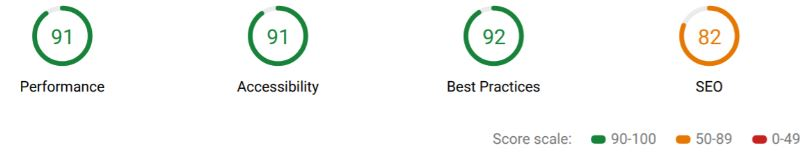
\includegraphics[width=\textwidth]{bereket/Lighthouse-rapport-ny-nettsted.png}
    \caption{Resultater fra Google Lighthouse}
    \label{fig:analysis-current-lightouse-summary}
\end{figure}

\subsubsection{Checkbot}
Oppsummering av resultatene etter testing med  Checkbot viser en god poengsum i gjennomsnitt. Den tester SEO, hastighet og sikkerhet.
\begin{figure}[H]
    \centering
    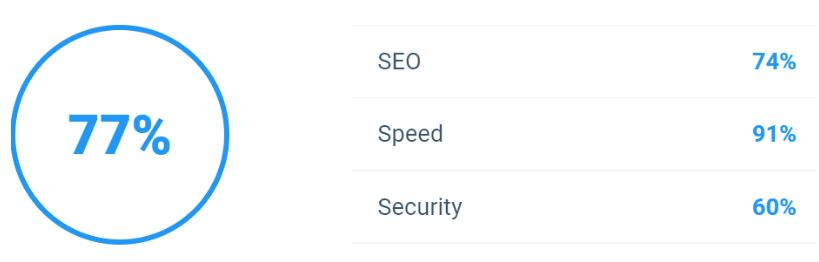
\includegraphics[width=\textwidth]{bereket/Checkbot-test-ny-nettsted.png}
    \caption{Resultater fra checkbot}
    \label{fig:analysis-current-lightouse-summary}
\end{figure}

\subsubsection{Color Contrast Analyser}
\begin{figure}[H]
    \centering
    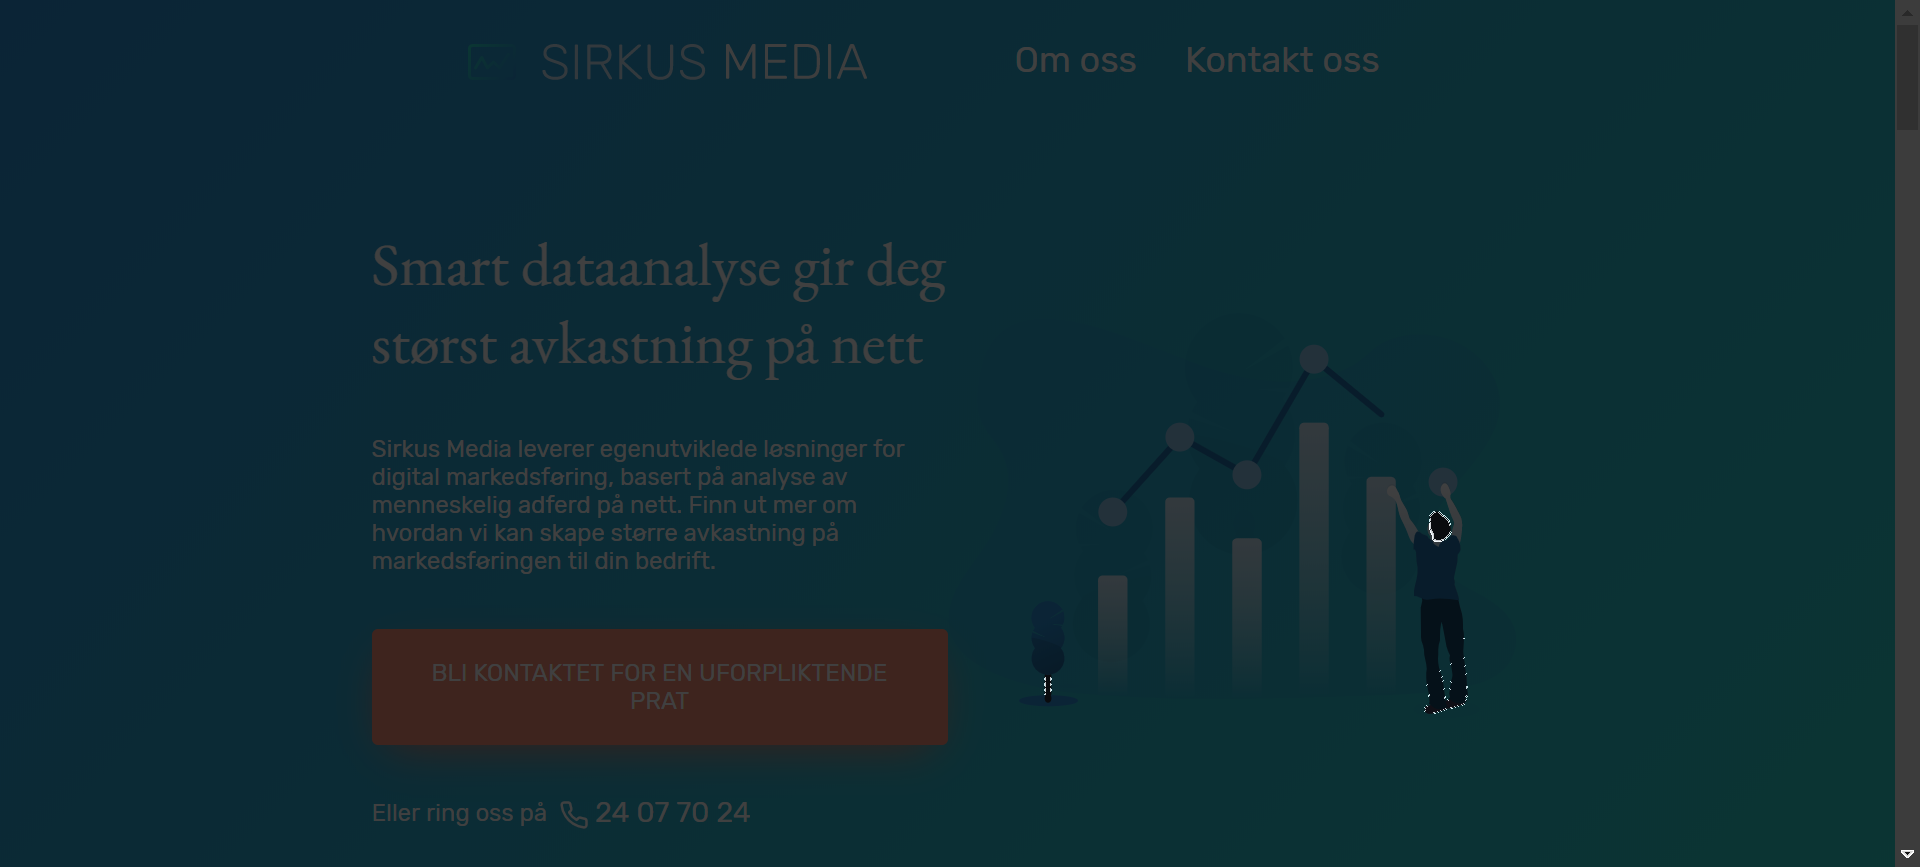
\includegraphics[width=\textwidth]{bereket/contrast-wcag-aa-small.png}
    \caption{Small non bold text for nivå AA}
    \label{fig:analysis-current-lightouse-summary}
\end{figure}
\begin{figure}[H]
    \centering
    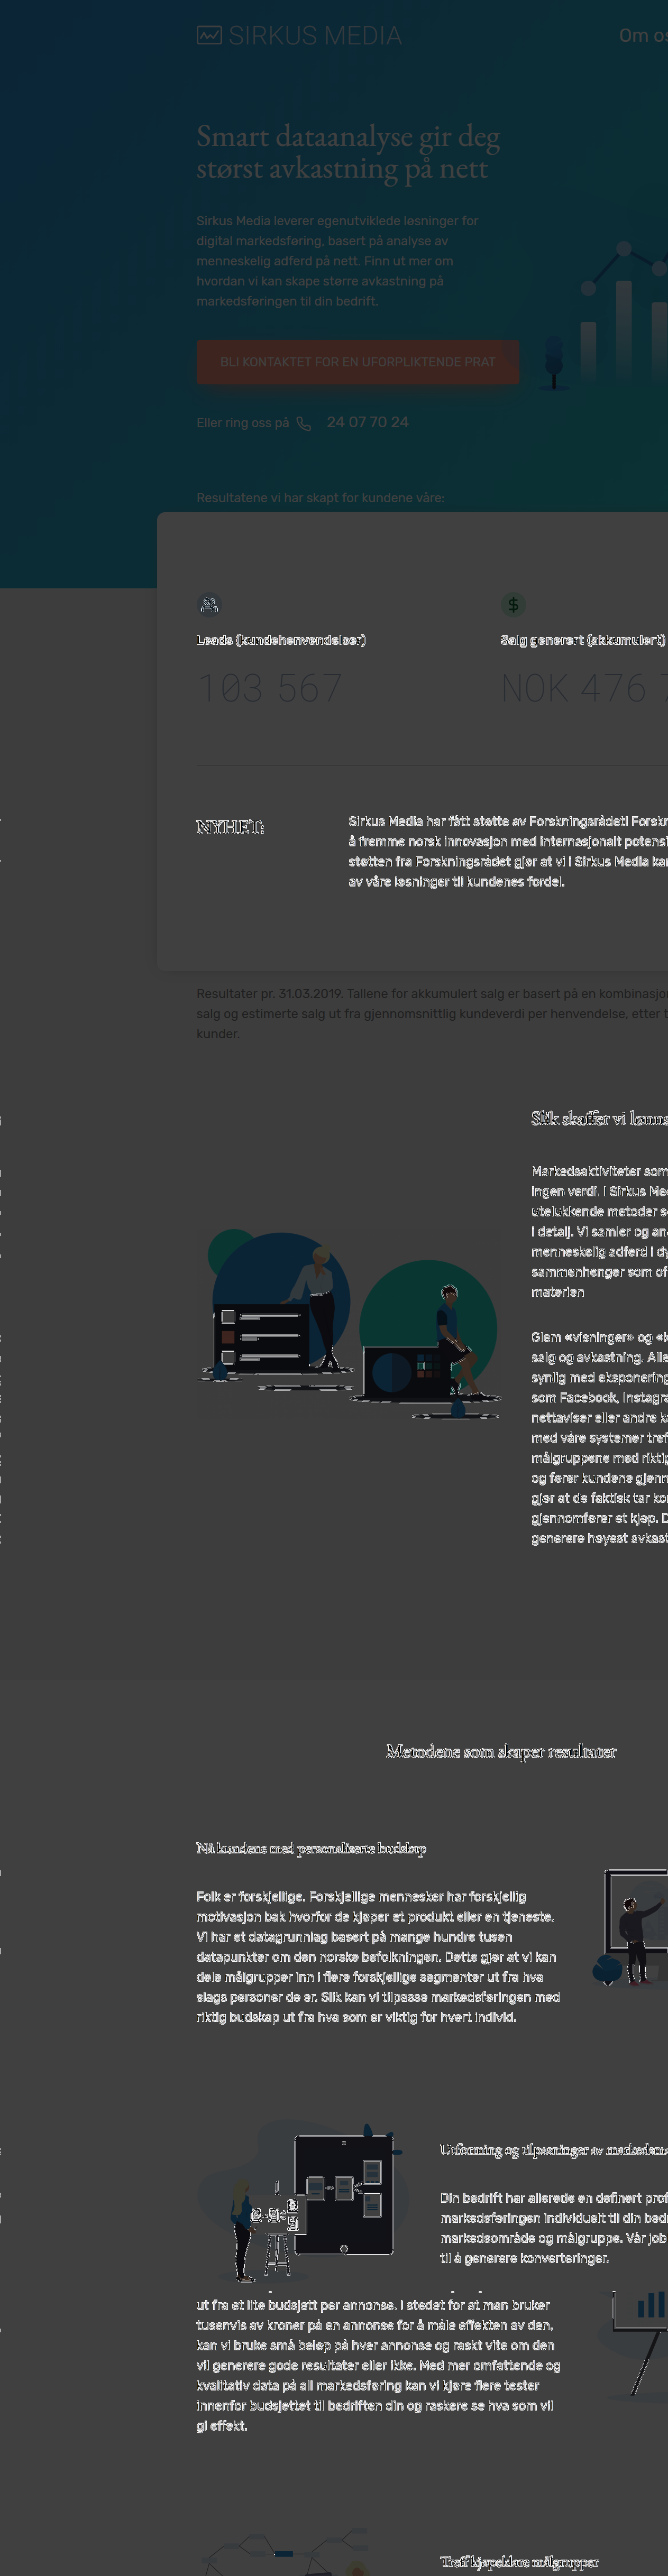
\includegraphics[width=\textwidth]{bereket/contrast-wcag-aaa-small.png}
    \caption{Small non bold text for nivå AAA}
    \label{fig:analysis-current-lightouse-summary}
\end{figure}

\subsubsection{WAVE}
Ved testing med wave ble det ingen feil. Det er bare to varslinger. Den ene varsler om det ikke finnes header-tag (h1-h6) og den andre handler om  javascript.

\begin{figure}[H]
    \centering
    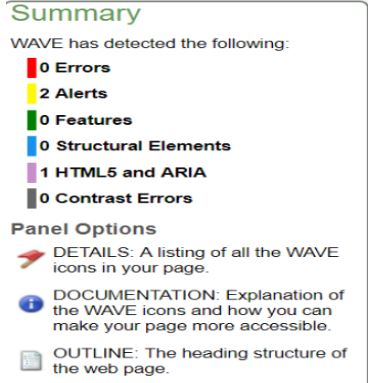
\includegraphics[width=\textwidth]{bereket/Wave-test-ny-nettsted.png}
    \caption{Resultat fra WAVE}
    \label{fig:analysis-current-lightouse-summary}
\end{figure}

\begin{figure}[H]
    \centering
    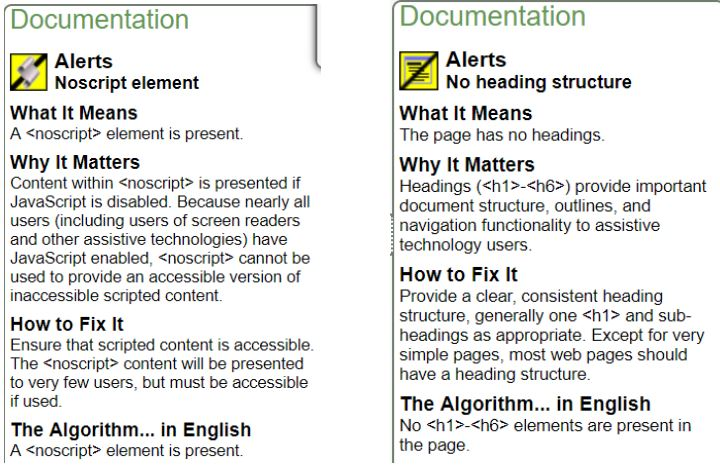
\includegraphics[width=\textwidth]{bereket/Wave-test-varsel-ny-nettsted.png}
    \caption{Varslinger fra WAVE}
    \label{fig:analysis-current-lightouse-summary}
\end{figure}

\subsubsection{Kontrastforhold mellom tekst og bakgrunn}
Brukte Google Chrome DevTools for å teste kontastforhold mellom tekst og bakgrunn og viser resultatet på bildet. Noen av tekstene er  ikke oppfyller kontrast kravet for AA og AAA. 
\begin{figure}[H]
    \centering
    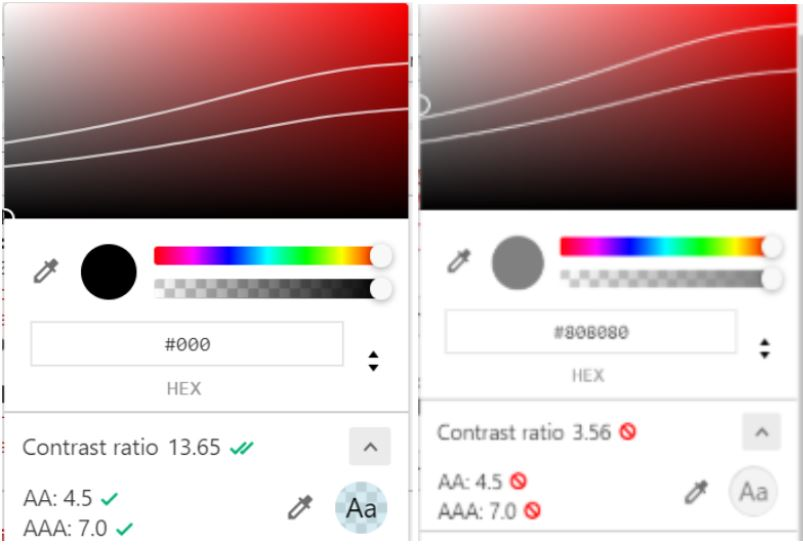
\includegraphics[width=\textwidth]{bereket/Kontrast-test.png}
    \caption{Varslinger fra WAVE}
    \label{fig:analysis-current-lightouse-summary}
\end{figure}

\subsubsection{Qualys SSL Server Test}
Resultatet etter testing med Qualys SSL Server viser en A+. Nåværende nettsiden viser A og blir forbedret til A++. 
\begin{figure}[H]
    \centering
    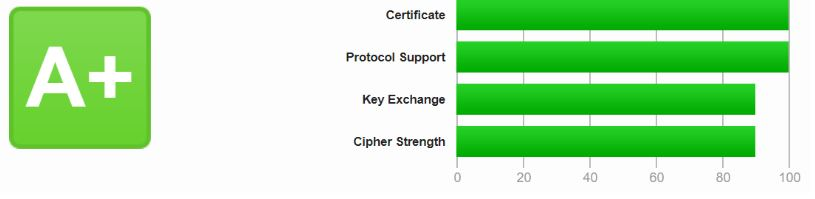
\includegraphics[width=\textwidth]{bereket/QSST-test.png}
    \caption{Sertifikat score}
    \label{fig:analysis-current-lightouse-summary}
\end{figure}
\subsubsection{Test med skjermleser}
Nettsiden ble testet med skjermleser (Ease of Access). Det er enkelt  å navigere seg rundt på nettsiden og innholdet kommer i en logisk rekkefølge. (Skip til innhold?) 

\subsubsection{Konklusjon}
Etter at vi tok en test med Google Chrome DevTools, Google Lighthouse og Checkbot og så resultatet, kan vi si at nettsiden er rask. Når vi sammenligner testresultatet fra nåværende nettsiden og den nye nettsiden, har den nye nettsiden fått bedre score i de fleste tilfeller. Ved testing med Google Lighthouse får den nye nettsiden fikk bedre resultat på ytelse, beste praksis og tilgjengelighet. I SEO fikk nåværende nettsiden bedre resultat. Grunnen til dette er at dagens nettsted består av kun en forside og lite informasjon. Dette begrenser muligheten for feil. 
Checkbot testresultatet viser at 77\% i gjennomsnitt på den nye nettsted, mens dagens nettsted scoret 70\%. 
WAVE rapporterer om 20 kontrastfeil, 1 dokument språk mangler, 4 tomme linker og 5 redudante linker på dagens nettsiden og ingen feil på den nye.
Qualys SSL Server Test viser A på dagens nettsted og A+ på den nye nettsted.

Full rapport for Google Lighthouse testen kan leses i vedlegg X (KOMMER).

\clearpage